
\documentclass[compress]{beamer}

%\usepackage{beamerthemesplit}
\usepackage{xmpmulti}

\usepackage{graphicx,float,wrapfig, bbm}
\usepackage{amsfonts, bbold, comment}
\usepackage{mdwlist}
\usepackage{subfigure}
\usepackage{colortbl}

\usepackage{multirow}

\pgfdeclareimage[width=\paperwidth]{mybackground}{colorado/boulder.pdf}

\newcommand{\fsi}[2]{
\begin{frame}[plain]
\vspace*{-1pt}
\makebox[\linewidth]{\includegraphics[width=\paperwidth]{#1}}
\begin{center}
#2
\end{center}
\end{frame}
}


\newcommand{\e}[2]{\mathbb{E}_{#1}\left[ #2 \right] }
\newcommand{\ind}[1]{\mathbb{I}\left[ #1 \right] }
\newcommand{\ex}[1]{\mbox{exp}\left\{ #1\right\} }
\newcommand{\g}{\, | \,}
\newcommand{\citename}[1]{#1 }

\newcommand{\gfxs}[2]{
\begin{center}
	\includegraphics[width=#2\linewidth]{simtrans/#1}
\end{center}
}

\newcommand{\gfxq}[2]{
\begin{center}
	\includegraphics[width=#2\linewidth]{qb/#1}
\end{center}
}


\usetheme[bullet=circle,                     % Use circles instead of squares for bullets.
          titleline=true,                    % Show a line below the frame title.
          showdate=true,                     % show the date on the title page
          alternativetitlepage=true,         % Use the fancy title page.
          titlepagelogo=general_figures/culogo,              % Logo for the first page.
          % Logo for the header on first page.
          headerlogo=general_figures/boulder_cs,
          ]{UCBoulder}

\usecolortheme{ucdblack}
\title[Thinking on Your Feet]{Thinking on your Feet: \\ Atlanta HSNCT Exhibition Match}
\author{ Jordan Boyd-Graber}
\date{May 27, 2017}

\institute[Boulder] % (optional, but mostly needed)
{University of Colorado Boulder}

\begin{document}

\frame{
\titlepage
\tiny
}

\section{Introduction}

\begin{frame}{The Competition}

\begin{itemize}
	\item A computer that plays quiz bowl: \textsc{qanta}
        \item <2->{{\bf Q}uestion {\bf A}nswering is {\bf N}ot a {\bf T}rivial {\bf A}ctivity}
	\item Facing off against top quiz bowlers
          \only<3->{
	\item But first
	\begin{itemize}
		\item Who we are
                \item Why quiz bowl is interesting scientifically
		\item Explaining what's going to happen
                \item Connection to hard real-world problems
	\end{itemize}}
\end{itemize}

\end{frame}

\begin{frame}{Who we are}


	\begin{columns}
		\column{.5\linewidth}
                \begin{itemize}
                  \item \alert<1>{Jordan Boyd-Graber}
                  \item \alert<2>{Mohit Iyyer}
                  \item \alert<3>{Pedro Rodriguez}
                  \item \alert<4>{Shi Feng}
                   \item Hal Daum\'e III
                   \item He He
                   \item Kevin Kwok
                   \item \dots
                \end{itemize}


		\column{.5\linewidth}

                \only<1>{
			\begin{block}{Jordan Boyd-Graber}

			\begin{itemize}
				\item Professor at Colorado (returning
                                  to UMD in Fall)
				\item Former quiz bowl player at Caltech (4$^{th}$, 2004 UG ICT) and Princeton (4$^{th}$, ACF Nats 2005)
			\end{itemize}
			\gfxq{jordan_qb}{.5}
			\end{block}
			}


\only<2>{
			\begin{block}{Mohit Iyyer}
			\begin{itemize}
				\item Next week: Dr. Iyyer
                                \item Next month: AI$^2$
                                \item Next year: Assistant Professor
                                  at U Mass Amherst
				\item National Champion, 2008 HSNCT
			\end{itemize}
			\gfxq{mohit_qb}{.5}
			\end{block}
}

\only<3>{
			\begin{block}{Pedro Rodriguez}
			\begin{itemize}
				\item Second Year PhD Student
                                \item UC Boulder
                                 \item Guessing System
			\end{itemize}
			\gfxq{pedro}{.5}
			\end{block}
}

\only<4>{
			\begin{block}{Shi Feng}
			\begin{itemize}
				\item First Year PhD Student
                                \item UMD
                                \item Buzzing System
			\end{itemize}
			\gfxq{shi}{.5}
			\end{block}
}


	\end{columns}
\end{frame}


\section{QANTA}

\begin{frame}
	\frametitle{How is this different from Watson?}

	\begin{columns}
		\column{.5\linewidth}

		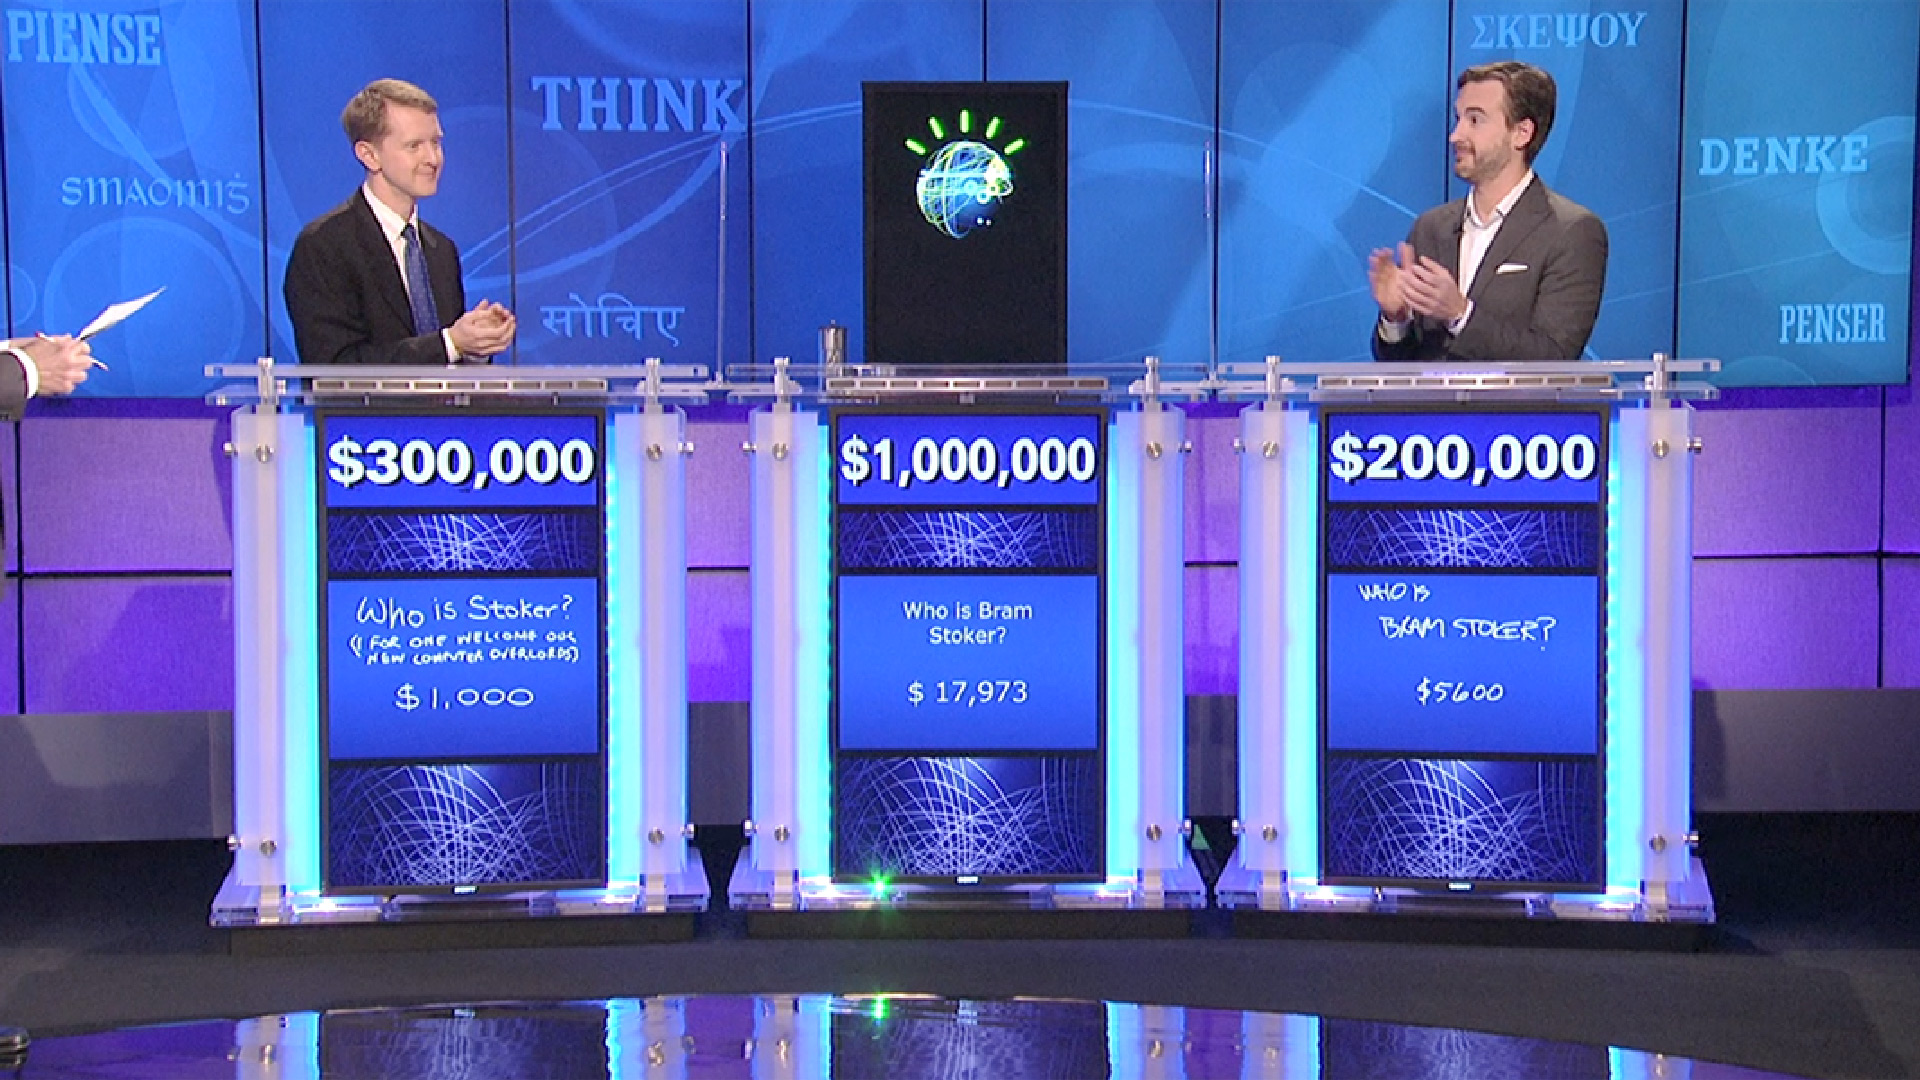
\includegraphics[width=1.0\linewidth]{qb/jeopardy}


		\column{.5\linewidth}
		\begin{itemize}
			\item This is {\bf not} Jeopardy
			\item There are buzzers, but players only buzz
                          at the question end
			\item Doesn't discriminate knowledge
			\item Quiz bowl is pyramidal
                        \item Watson must decide to answer {\bf once}, after
                          complete question
                        \item Quiz Bowl: decide after each word
                        \pause
                        \item We're not \textsc{ibm} / Google
		\end{itemize}

	\end{columns}

\end{frame}



\begin{frame}{Matching Entites Across Sentences}

\begin{block}{\only<2->{Magic Flute}}

    At its premiere, \alert<3>{the librettist of this opera} portrayed
    \alert<4>{a character who asks for a glass of wine with his dying wish}. \alert<4>{That
    character} in this opera is instructed to ring some bells to summon
    his love. At its beginning, \alert<5>{a man} who claims to have killed a (*)
    serpent has a padlock put on \alert<5>{his} mouth because of \alert<5>{his} lying. The
    plot of this opera concerns a series of tests that \alert<5>{Tamino} must
    undergo to rescue Tamina from Sorastro. For 10 points, name this
    Wolfgang Mozart opera titled for \alert<6>{an enchanted woodwind instrument}.
\end{block}



\only<3-4>{{\bf Not all references are named (\alert<3>{Emanuel
      Schikaneder}, \alert<4>{Papageno})}}
\only<5>{Need to be able to match pronouns across sentences (or have
  deep world knowledge)}
\only<6>{Requires semantic knowledge}
\end{frame}


\begin{frame}{How the shared task works}

\begin{columns}

  \column{.65\linewidth}
  \begin{itemize}
    \item<2-> 1. I’m User #1.  I’d like to play!
    \item<4-> I’d like to hear the Word~1 of Question 1
    \item<6-> I’d like to hear the Word~2 of Question 1
    \item<8-> I’d like to hear the third word of Question 1
    \item<10-> I’d like to answer Question 1 with \texttt{Barry_Goldwater}
  \column{.3\linewidth}
  \gfxq{buzzer}{.8}
\end{columns}

\begin{columns}


  \column{.3\linewidth}
  \gfxq{bamber}{.8}

  \column{.65\linewidth}
  \begin{itemize}
    \item<3-> Hi! Available questions are \texttt{[1,2,3,4]}
    \item<5-> It's \texttt{Extremism}
    \item<7-> It's \texttt{in}
    \item<9-> It's \texttt{the}
    \item<11-> It's \texttt{defense}
    \item<13-> Got it, thanks!  You've answered Question 1 at Position
      3 with \texttt{Barry_Goldwater}
  \end{itemize}

\end{columns}


\end{frame}


\begin{frame}{Vector Space Model}

  \only<1>{\gfxq{unigram_models_0}{.8}}
  \only<2>{\gfxq{unigram_models_1}{.8}}
  \only<3>{\gfxq{unigram_models_2}{.8}}
  \only<4>{\gfxq{unigram_models_3}{.8}}
  \only<5>{\gfxq{unigram_models_4}{.8}}
  \only<6>{\gfxq{unigram_models_5}{.8}}
  \only<7>{\gfxq{unigram_models_6}{.8}}
  \only<8>{\gfxq{unigram_models_7}{.8}}
  \only<9>{\gfxq{unigram_models_8}{.8}}


\end{frame}

\begin{frame}{How to approach this problem \dots}

    \only<1>{
  \begin{columns}
    \column{.5\linewidth}
    \gfxq{guess}{0.8}
    \column{.5\linewidth}
    \gfxq{buzzer}{0.8}
  \end{columns}
}
\only<2>{
   \gfxq{buzzer}{0.5}
}
\end{frame}


\begin{frame}
\frametitle{How we know how we're doing}

\begin{columns}

	\column{0.5\linewidth}

	\begin{center}
		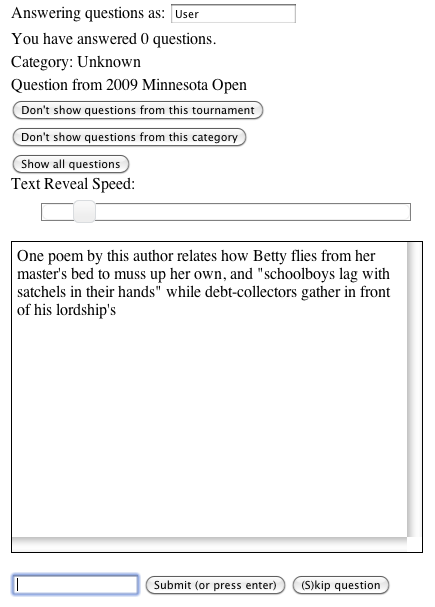
\includegraphics[width=0.8\linewidth]{qb/screenshot}
	\end{center}

	\column{0.5\linewidth}


	\only<2>{
	\begin{itemize}
		\item Similar to Quizzy Google Wave app
                \item Launched 2011
                \item Imitated / improved by Protobowl (who became
                  coauthors on our papers)
	\end{itemize}
        \gfxq{protobowl}{.8}
	}

\end{columns}
\end{frame}


\begin{frame}{Not all opponents are equal}

  \gfxq{player_profile}{.9}


\end{frame}

\begin{frame}{Know when to Buzz 'em}

  \only<1>{\gfxq{error1}{.8}}
  \only<2>{\gfxq{error2}{.8}}
  \only<3>{\gfxq{error3}{.8}}
  \only<4>{\gfxq{error4}{.8}}
  \only<5>{\gfxq{error5}{.8}}
  \only<6>{\gfxq{error6}{.8}}

  Deep Reinforcement Opponent Network (ICML 2016)

\end{frame}





\begin{frame}{What you'll see}
  \only<3->{\gfxq{interface_score}{.8}}
  \only<2->{\gfxq{interface_question}{.8}}
  \only<1->{\gfxq{interface_guess}{.8}}
\end{frame}


\begin{frame}{It's not all fun and games \dots}

  \begin{columns}
    \column{.4\linewidth}
    \begin{center}
        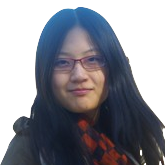
\includegraphics[width=0.7\linewidth]{general_figures/hehe} \\
        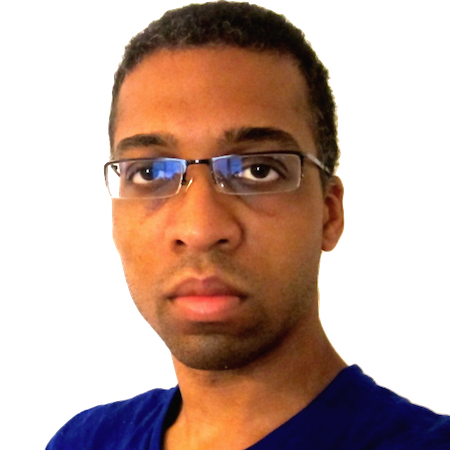
\includegraphics[width=0.7\linewidth]{general_figures/alvin}
      \end{center}
    \column{.6\linewidth}
        \begin{block}{ {\bf \href{http://cs.colorado.edu/~jbg/docs/2015_emnlp_rewrite.pdf}{Syntax-based Rewriting for Simultaneous Machine Translation}}}
He He, Alvin Grissom II, {\bf Jordan Boyd-Graber}, and Hal {Daum\'{e} III}.  \emph{Empirical Methods in Natural Language Processing}, 2015
        \end{block}

\begin{block}{ {\bf \href{http://cs.colorado.edu/~jbg/docs/2014_emnlp_simtrans.pdf}{Don't Until the Final Verb Wait: Reinforcement Learning for Simultaneous Machine Transl\
ation}}}
\underline{\href{http://www.umiacs.umd.edu/~alvin/}{Alvin Grissom II}}, {\bf Jordan Boyd-Graber}, He He, John Morgan, and Hal {Daum\'{e} III}.  \emph{Empirical Methods in Natural L\
anguage Processing}, 2014
        \end{block}
  \end{columns}
\end{frame}

\begin{frame}{Why simultaneous translation hard is}

  \begin{columns}
    \column{.5\linewidth}
       \gfxs{nuremberg_translators}{.9}
    \column{.5\linewidth}
       \begin{itemize}
         \item Languages like German and Japanese are {\bf verb final}
         \item {\bf Guess} what the verb will be
         \item Know when you're right about verb ({\bf Buzz})
       \end{itemize}
  \end{columns}

\end{frame}

\section{Competition}

\begin{frame}{Inconclusive First Steps}

		\begin{columns}
			\column{.25\linewidth}
				\gfxq{colby_jeo}{1.0}
                                Colby Burnett:
                                \$375,000
			\column{.25\linewidth}
				\gfxq{ben_jeo}{1.0}
                                Ben Ingram:
                                \$427,534
			\column{.25\linewidth}
				\gfxq{alex_jeo}{1.0}
                                Alex Jacobs: \$151,802
			\column{.25\linewidth}
				\gfxq{kristin_jeo}{1.0}
                                Kristin Sausville: \$95,201
		\end{columns}

                \pause

                \begin{center}
                End result: 200-200 tie!
                \end{center}

\end{frame}

\fsi{qb/hsnct1}{}
\fsi{qb/jennings}{23. October 2015, Seattle}
\fsi{qb/jennings_handshake}{300-160}
\fsi{qb/nasat}{Humans 345-145}
\fsi{qb/hsnct_2016}{Humans 190-155}



\begin{frame}{}

	\begin{center}
	\begin{Huge}
	The Match! \\
	\end{Huge}
        \begin{itemize}
          \item 40 tossups (from earlier today)
          \item No bonuses
          \item Off the clock
        \end{itemize}

        \pause
        QA Afterward
	\end{center}

\end{frame}


\begin{frame}{We want (and need) your help!}

	\begin{itemize}
		\item Our system isn't perfect
		\item We need more data
		\item We need more features
		\item We need excellent coders
	\end{itemize}

	\pause

	\begin{block}{Find out more \dots}
		\begin{itemize}
			\item Code: \url{http://github.com/Pinafore/qb}
			\item Twitter: @boydgraber
			\item Announcements on HSQB
                        \item Shared Task \url{https://sites.google.com/view/hcqa}
		\end{itemize}
	\end{block}

\end{frame}

\begin{frame}{Postmortem}

What we tried to improve \dots
\begin{itemize}
	\item Tried to make system more aggressive
        \item Vastly increased answer set (important for Trash)
        \item Faster training time (AWS)
\end{itemize}
\end{frame}


\begin{frame}{Come to UMD}

\begin{columns}
	\column{.5\linewidth}
        \only<1>{
        	\begin{center}
		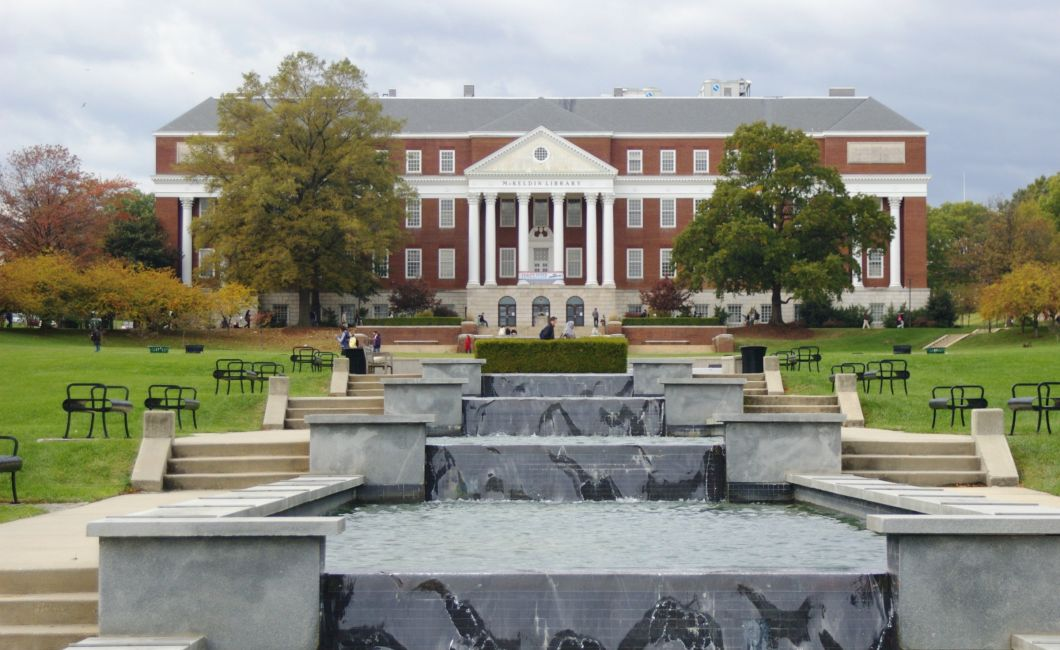
\includegraphics[width=.9\linewidth]{umd/umd} \\
		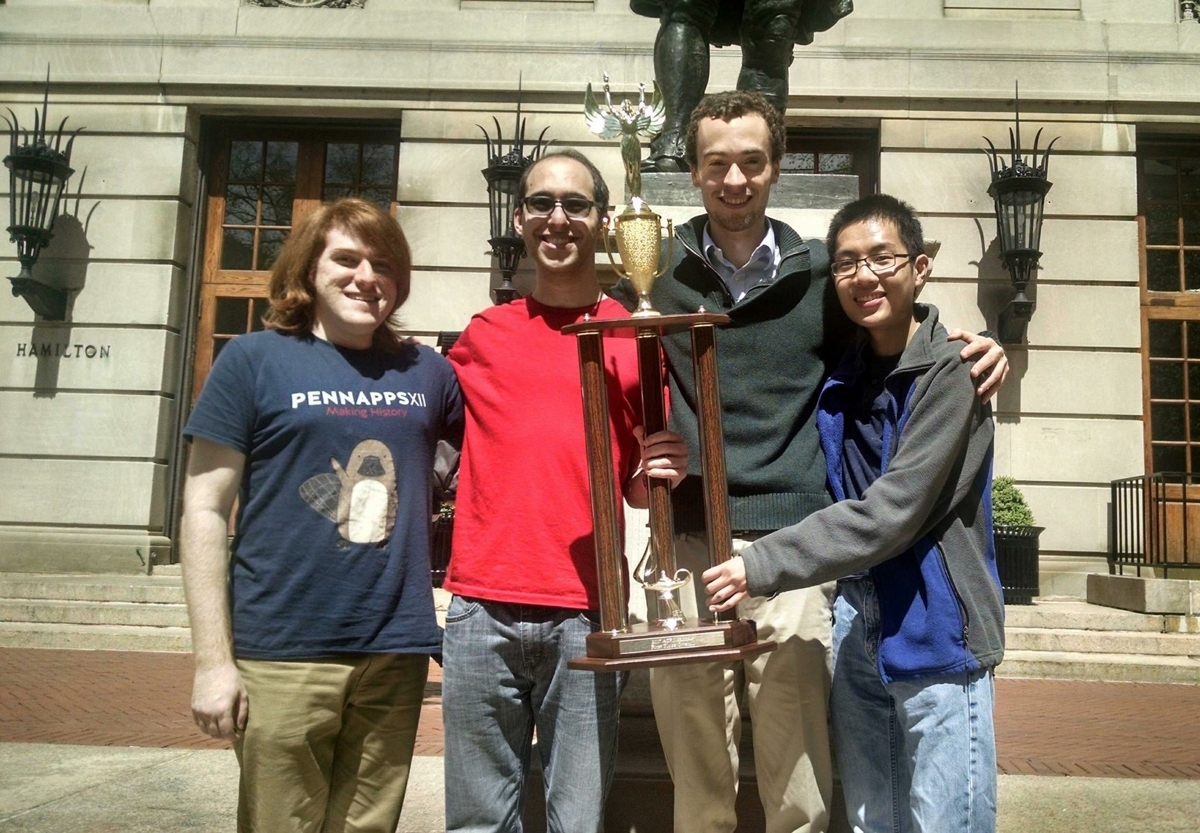
\includegraphics[width=.9\linewidth]{umd/qb_team}
	\end{center}
              }
	\column{.5\linewidth}
		\begin{itemize}
                \item Looking for undergrads/grads/interns
                \item A great place for natural language
                  processing and machine learning
                \item Not too shabby at quiz bowl either
		\end{itemize}
\end{columns}

\end{frame}


\frame{

	\frametitle{Thanks}

        \begin{block}{Collaborators}
          \textsc{naqt}, Pedro Rodriguez (Colorado), Shi Feng (UMD),
          Mohi Iyyer (UMD), Vivian Lai (Colorado), Hal Daum\'e III (UMD), Anupam Guha
          (Maryland), Manjhunath Ravi (Colorado), Danny Bouman (UMD
          UG),
          Stephanie Hwa (UMD UG),
        \end{block}

        \begin{block}{Funders}
        \begin{center}
          
\includegraphics[width=0.3\linewidth]{general_figures/nsf}
       \end{center}
        \end{block}
}



\end{document}
